
\section{Class 5 - Independence, Chebyshev's, Bernoullis, and Binomials}

\subsection{Independence of Random Variables}

We previously introduced independence of events. We now discuss independence of random variables.

\begin{remark}
    We use the following notational short hand
    \[
    P(X = x, Y = y) = P( \{ X = x \} \cap \{ Y = y \}  )
    \]
\end{remark}


\begin{definition}[Independence]
    Let $X, Y$ be discrete random variables on $\Omega$. We say that $X$ and $Y$ are \textbf{independent} if 
    \[
        P(X = x, Y = y) = P( \{ X = x \} \cap \{  Y = y \}  )  = P(X = x) P(Y = y)
    \] for every $x$ and $y$.
\end{definition}

\begin{result}[Expectation of product of independent random variables]
    Let $X, Y$ be discrete random variables on $\Omega$ with $\operatorname{supp}(X) = A , \operatorname{supp}(Y)  = B$. If $X, Y$ independent, then 
    \[
        \mathbb{E}\left[ XY\right]  = \mathbb{E}\left[ X\right] \mathbb{E}\left[ Y\right] 
    \]

    This is denoted
    \[
    X \perp Y
    \]
\end{result}

\begin{proof}
    \begin{align*}
        \mathbb{E}\left[ XY\right]  
        &= \sum\limits_{x \in A}^{}  \sum\limits_{y \in B}^{}  x \cdot y P (X = x, Y = y) \quad \text{ by definition of expectation} \\
        &= \sum\limits_{x \in A}^{}  \sum\limits_{y \in B}^{}  x \cdot y P (X = x) P(Y = y) \quad \text{ by independence} \\
        &= \left( \sum\limits_{ x \in A}^{}x P(X = x)  \right)  \left( \sum\limits_{y \in B}^{}y P(Y = y)  \right)  \\
        &= \mathbb{E}\left[ X\right]  \mathbb{E}\left[ Y\right]  \text{ by definition of expectation}
    \end{align*}
\end{proof}

\begin{remark}
    Note that the implication only works one way 
    \[
    X \perp Y \implies \mathbb{E}\left[ XY\right]  = \mathbb{E}\left[ X\right]  \mathbb{E}\left[ Y\right] 
    \]
    The converse is not true 
    \[
        \mathbb{E}\left[ XY\right]  = \mathbb{E}\left[ X\right]  \mathbb{E}\left[ Y\right] \not \Rightarrow X \perp Y 
    \]
    
\end{remark}

\subsection{Chebyshev's Inequality}

Chebyshev's allows us to bound the probability that a random variable deviates by a \textit{certain amount} from its mean.

\begin{theorem}[Chebyshev's Inequality]
    Let $X$ be a random variable with expectation $\mu$ and variance $\sigma^2$. For any $t > 0$,
    \[
    P \left(  \left| X - \mu \right| \geq t \right)  \leq \frac{\sigma^2}{t^2}
    \]
\end{theorem}

\subsection{Bernoulli Random Variable}

\begin{remark}
    For random variable $X$, we sometimes use the following short hand 
    \[
        P_X(x) = P(X = x)
    \]
\end{remark}


\begin{definition}[Bernoulli] 
    A random variable $X : \Omega \to \{ 0, 1 \} $ is a \textbf{Bernoulli} random variable with parameter $p \in [0, 1]$ if 
    \[
    P_X(1) = p, \quad P_X(0) = 1 - p
    \]
    We denote this 
    \[
        X \sim \operatorname{Bern} (p)
    \]
\end{definition}

\begin{result}[Moments of a Bernoulli random variable]

    The mean of a Bernoulli is  
    \[
    \mathbb{E}\left[ X\right]  = 1 \cdot p + 0 \cdot ( 1- p) = p
    \]

    To find $\mathbb{E}\left[ X^2\right] $
    \begin{align*}
        \mathbb{E}\left[ X^2\right]  &= \sum\limits_{x \in \{ 0, 1 \} }^{} x^2 P(X = x) \\
        &= 1 \cdot p + 0 \cdot ( 1-p) \\
        &= p
    \end{align*}
    

    The variance of a Bernoulli is 
    \begin{align*}
        \operatorname{Var} (X) &= \mathbb{E}\left[ X^2\right]  - \mathbb{E}\left[ X \right]^2 \\
        &= p - p^2
    \end{align*}
\end{result}

\begin{remark}
    The maximum variance of a Bernoulli random variable is achieved when $p = \frac{1}{2}$

\begin{center}
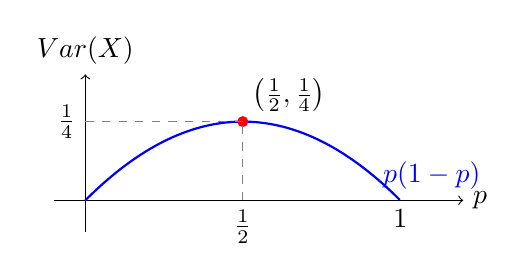
\begin{tikzpicture}[scale=4]
    % Axes
    \draw[->] (-0.1,0) -- (1.2,0) node[right] {$p$};
    \draw[->] (0,-0.1) -- (0,0.4) node[above] {$\operatorname{Var}(X)$};

    % Variance curve p(1-p)
    \draw[thick, blue, domain=0:1, samples=100] plot (\x, {\x*(1-\x)});

    % Maximum point at p = 1/2
    \fill[red] (0.5, 0.25) circle (0.5pt);
    \node[above right] at (0.5, 0.25) {$\left(\frac{1}{2}, \frac{1}{4}\right)$};

    % Dashed lines to axes
    \draw[dashed, gray] (0.5, 0) -- (0.5, 0.25);
    \draw[dashed, gray] (0, 0.25) -- (0.5, 0.25);

    % Tick marks
    \node[below] at (0.5, 0) {$\frac{1}{2}$};
    \node[below] at (1, 0) {$1$};
    \node[left] at (0, 0.25) {$\frac{1}{4}$};

    % Label for curve
    \node[blue] at (1.1, 0.08) {$p(1-p)$};
\end{tikzpicture}
\end{center}
\end{remark}

\subsection{Binomial Random Variable}

\begin{definition}
    [Binomial Random Variable]
    Let $X_1, \hdots X_n$ be independent Bernoullis with the same parameter $p \in [0, 1]$. A \textbf{binomial} random variable $S_n$ with parameter $n, p$ is defined as 
    \[
        S_n = \sum\limits_{i = 1}^{n} X_i
    \]
    $S_n$ takes as its support $\{  0, 1, \hdots n \} $. \\

    $S_n$ has pmf
    \[
    P(S_n = x) = \begin{cases}
        \binom{n}{x} p^x (1 - p)^{n - x} & \text{if } x \in \operatorname{supp}(S_n) \\
        0 & \text{otherwise}
    \end{cases}
    \]
    We denote this 
    \[
    S_n \sim \operatorname{Binom} (n, p)
    \]
\end{definition}

\begin{proof}
    We want to show for $x \in \operatorname{supp}(S_n) $,
    \[P(S_n = x) = \binom{n}{x} p^x (1-p)^{n-x}
    \]

    Fix $x \in \operatorname{supp}(S_n) $. An outcome with exactly $x$ successes is an unordered collection of $x$ successes and $n - x$ failures. Each ordered sequence with $x$ successes is equally likely. \\

    The probability of getting an ordered sequence of $x$ successes followed by $n-x$ failures is, by independence,
    \[
        p^x (1-p)^{n-x}
    \]
    The number of such sequences is the number of ways to choose $x$ positions in $n$ to be successes
    \[
        \binom{n}{x}
    \]

    Hence the pmf is
    \[
        P(S_n = x) = \binom{n}{x} p^x (1-p)^{n-x}
    \]
\end{proof}


\begin{remark}
    A binomial random variable with parameter $n, p$ counts the number of successes in $n$ independent and idential trials, each with success probability $p$.
\end{remark}

\begin{result}[Moments of Binomial random variables]
    The mean of a binomial random variable is 
    \begin{align*}
        \mathbb{E}\left[ S_n\right]  &= \mathbb{E}\left[ 
            \sum\limits_{i = 1}^{n}  X_i
        \right] \quad \text{by definition}\\
        &= \sum\limits_{i = 1}^{n}  X_i \quad \text{by linearity of expectation} \\
        &= \sum\limits_{i = 1}^{n}  p \\
        &= np
    \end{align*}
    To find $\mathbb{E}\left[ S_n^2\right] $
    \begin{align*}
        \mathbb{E}\left[ S_n^2\right] &= \mathbb{E}\left[ 
            \left( \sum\limits_{i = 1}^{n} X_i \right)^2 
        \right]  \\
        &= \mathbb{E}\left[ 
            (X_1 + X_2 + \hdots X_n)^2
        \right]  \\
        &= \mathbb{E}\left[ 
            \sum\limits_{i = 1}^{n}  X_i^2 
            + 
            \sum\limits_{ i \neq j}^{}  X_i X_j
        \right] \\
        &= \sum\limits_{i = 1}^{n}  \mathbb{E}\left[ X_i^2\right]  + \sum\limits_{i \neq j}^{}  \mathbb{E}\left[X_i X_j \right] \quad \text{by linearity} \\
        &= \sum\limits_{i = 1}^{n}  \mathbb{E}\left[ X_i^2\right]  + \sum\limits_{i \neq j}^{}  \mathbb{E}\left[X_i \right] \mathbb{E}\left[ X_j\right]  \quad \text{by independence of $X_i, X_j$} \\ 
        &= \sum\limits_{i = 1}^{n} p  + \sum\limits_{i \neq j}^{} p^2\\
        &= np + n(n-1) p \\
    \end{align*}

    Hence the variance of $S_n$ is 
    \begin{align*}
        \operatorname{S_n}  &= \mathbb{E}\left[ S_n^2\right]  - \mathbb{E}\left[ S_n\right]^2 \\
        &= np + n(n-1)p - (np)^2 \\
        &= np(1-p)
    \end{align*}
\end{result}

\begin{remark}
    To see how we expand $(X_1 + X_2 + \hdots + X_n)^2$, consider the multiplication table:
    \[
    \begin{array}{c|cccc}
         \times & X_1 & X_2 & \cdots & X_n \\
        \hline
        X_1 & \boxed{X_1^2} & X_1 X_2 & \cdots & X_1 X_n \\
        X_2 & X_2 X_1 & \boxed{X_2^2} & \cdots & X_2 X_n \\
        \vdots & \vdots & \vdots & \ddots & \vdots \\
        X_n & X_n X_1 & X_n X_2 & \cdots & \boxed{X_n^2}
    \end{array}
    \]

    The sum of all entries in this $n \times n$ table gives $(X_1 + \hdots + X_n)^2$:
    \begin{itemize}
        \item {Diagonal entries}: $n$ terms
        \item {Off-diagonal entries}: $n(n-1)$ terms, there are a few ways to see this
        \begin{itemize}
            \item $n^2 - n$ terms, by counting total terms - $n$ diagonal terms 
            \item ${}_n P_2$ terms, by counting number of ways to permute $2$ out of $n$ 
            \item $2 \cdot {}_n C_2 = 2 \binom{n}{2}$ terms, by counting number of ways to choose $2$ out of $n$ terms, and then permuting the 2 terms
        \end{itemize} 
    \end{itemize}

    Hence
    \[
        (X_1 + X_2 + \hdots + X_n)^2 = \underbrace{\sum_{i=1}^{n} X_i^2}_{n \text{ terms}} + \underbrace{\sum_{i \neq j} X_i X_j}_{n(n-1) \text{ terms}}
    \]
\end{remark}

\begin{remark}[Concentration of binomial]
    Let $S_n \sim \operatorname{Binom}(n, p) $

    \textbf{Intuition}: For a binomial \textit{most probability mass lies near the center}. \\

    When $p = \frac{1}{2}$
    
    \[P(S_n = k) = \binom{n}{k} \left( \frac{1}{2}\right)^{k} \left(\frac{1}{2}\right)^{n - k} = \binom{n}{k} 2^{-n}
    \]

    The binomial coefficient is biggest when $ k = \frac{k}{2}$
    
    We can quantify the extent to which the pmf \textit{concentrates around the center} this using mean, variance, and Chebyshev's. \\

    \textbf{Proof}: \\

    By Chebyshev's, for any positive $t$ 
    \begin{align*}
        P \left( \left| S_n - np \right| \geq t  \right)  \leq \frac{np(1-p)}{t^2}
    \end{align*}

    This inequality is not very meaningful is $n$ is very large and $t$ is small, in which case our LHS will be something bigger than 1. We already know for free that the probability is less than 1.\\

    Since we get to choose whatever $t$ we want, we pick a $t$ such that $t^2$ is \textit{roughly as big as} $n$. \\

    Pick $t^2 = c\cdot n$. Then 
    \begin{align*}
        P \left( \left| S_n - np \right| \geq \sqrt{ c \cdot n} \right)  \leq \frac{p (1-p)}{c}
    \end{align*}

    \textbf{Conclusion}: Deviations of $S_n$ on the order of $\sqrt{n}$ happens with non-neglegible probability.  \\

    \textbf{Example}: Say $p = \frac{1}{2}$, then $S_n$ deviates from $ \frac{n}{2}$ by about $ \frac{\sqrt{n}}{2}$
    \begin{itemize}
        \item $n = 100, \frac{\sqrt{n}}{2} = 5$, most outcomes will be in $[45, 55]$
        \item $n = 10,000, \frac{\sqrt{n}}{2} = 50$, most outcomes will be in $[4950, 5050]$
    \end{itemize} 

    In the symmetric case ($p = \frac{1}{2}$), 
    \[
    P \left( \left| S_n - \frac{n}{2} \right|  \geq t \right)  \leq \frac{n}{4t^2}
    \]
    Take $t = 5 \sqrt{n}$
    \[ 
    P \left( \left| S_n - \frac{n}{2} \right|  \geq 5 \sqrt{n} \right) \leq \frac{1}{100}
    \]
    \textit{For symmetric binomial, we have less than 1\% chance of seeing a deviation of more than $5 \sqrt{n}$}.
\end{remark}






\newpage